%!TEX root = thesis.tex


\chapter{Robustness}
\label{chapter4}

One of the primary requirements of reinforcement learning in robotics is to train agents that work safely and effectively on a physical system.
Because RL agents are usually initially trained in simulation, agents must be robust to parametric uncertainty and unmodeled dynamics in order to be successfully transferred from simulation to reality (sim-to-real)~\cite{Tobin:2017a,Al-Nima:2021a}. In the absence of physical systems to perform sim-to-real evaluation for this work, robustness was evaluated by simulating modeling error for the benchmark systems.
% \rph{the trained agents were evaluated by modifying the model with different dynamics that were not included in the model during training.}

% \begin{itemize}
%   \item Provide dynamical analysis of what happens to the system when the parameters are changes
%   \item How do natural frequencies/modes change
%   \item How do the non-RL components of the controller respond to this error?
%   \item Will I be able to make any generalizations? It will likely be empirical
% \end{itemize}

\section{Duffing Oscillator Robustness}
%
The performance of the duffing oscillator with modeling error is dependent on the sensitivity of the model-based elements and RL elements of the controllers. The model-based component of the controllers is:
%
\begin{equation}
    f(t) = k_nx_d + \beta_n x_d^3
\end{equation}
%
where $k_n$ is the nominal linear stiffness and $\beta_n$ is the nominal nonlinear stiffness. 
Figure~\ref{fig_chap4:duffing_robustness_fixed_gain} shows the mean reward for a range in modeling error for $k$, $\beta$, and damping ratio, $\zeta$. Since the fixed-gain components are dependent on the nominal stiffness values and were designed to result in zero steady-state error, modeling error in the stiffness values causes steady-state error in the RL-PD and RL-LA responses.
% Since the fixed-gain component of the RL-PD and RL-LA controllers are dependent on nominal values for the stiffness parameters, modeling error in $k$ and $\beta$ cause steady-state error in the response.
% The fixed-gain terms of the RL-PD and RL-LA controllers were designed to supply an input that resulted in zero steady-state error. Therefore, modeling error in the linear stiffness, $k$, and nonlinear stiffness, $\beta$, results in steady-state error in the response and reduces the reward.
This steady-state error can reduce the reward from the responses. However, the reward for modeling error of $k$ in Figure~\ref{subfig_chap4:duffing_k_robustness_fixed_gain} increases with positive modeling error. This is due to lower oscillation amplitude compared to responses with $k$ lower than the nominal value.
%
The reward trend with modeling error in $k$ are similar for the $\beta$ modeling error shown in Figure~\ref{subfig_chap4:duffing_Beta_robustness_fixed_gain}. The reward is lower for $\beta$ that is lower than nominal due to higher oscillation amplitude, but reward is higher for larger $\beta$ due to lower oscillation amplitude.
%
The rewards from the time responses with error in damping ratio are shown in Figure~\ref{subfig_chap4:duffing_zeta_robustness_fixed_gain}. The nominal damping ratio used during training was $\zeta=0.01$, indicated by the vertical dashed line. Damping ratio was not used to design the fixed-gain controller and modeling error in damping ratio does not cause steady-state error. Therefore, the mean reward increases with increasing damping ratio due to faster oscillation decay.
%
\begin{figure}[t]
    \centering
    \begin{subfigure}[b]{0.49\textwidth}
        \centering
        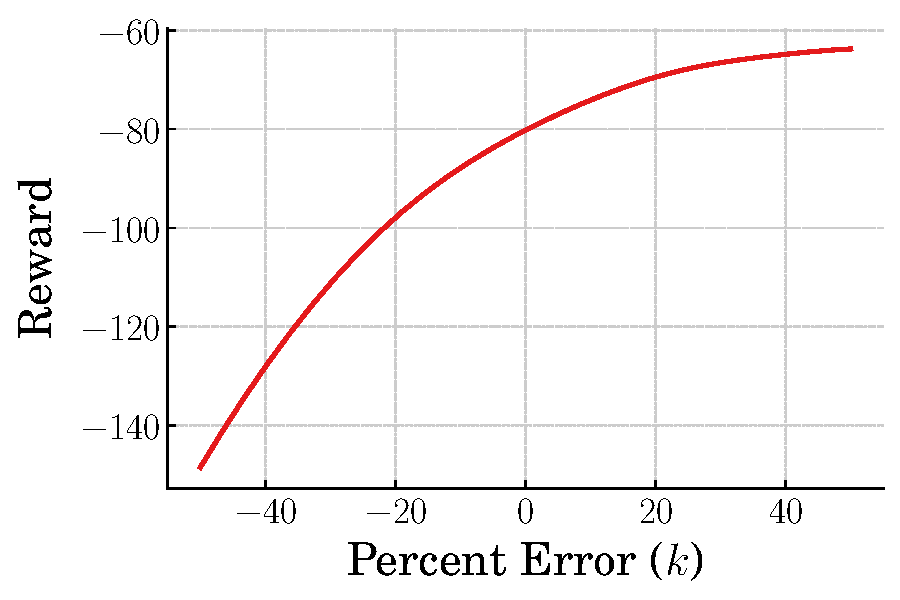
\includegraphics[width=\textwidth]{figures/figures_robustness/duffing_robustness/k_robustness_fixed_gain.pdf}
        \caption{$k$}
        \label{subfig_chap4:duffing_k_robustness_fixed_gain}
    \end{subfigure}\\
    \hfill
    \begin{subfigure}[b]{0.49\textwidth}
        \centering
        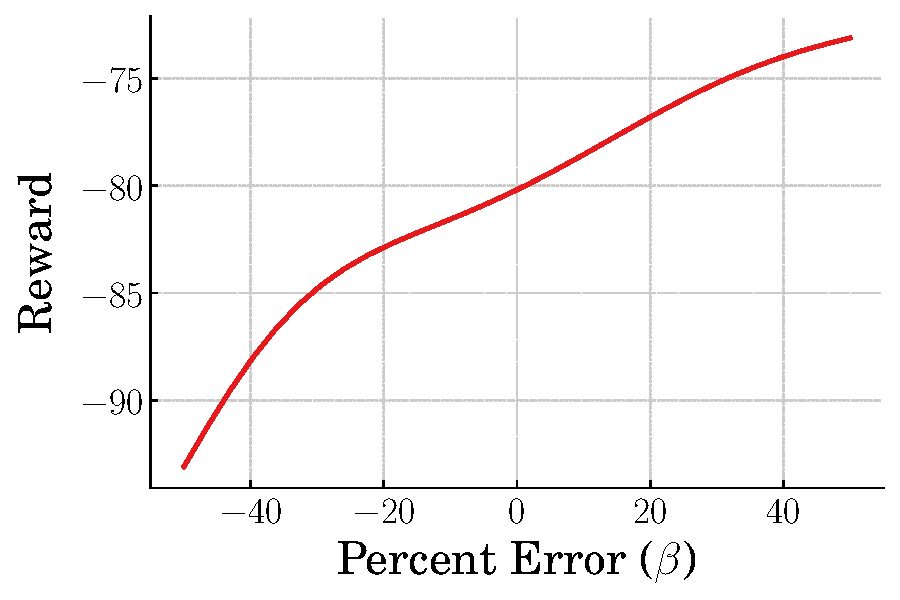
\includegraphics[width=\textwidth]{figures/figures_robustness/duffing_robustness/Beta_robustness_fixed_gain.pdf}
        \caption{$\beta$}
        \label{subfig_chap4:duffing_Beta_robustness_fixed_gain}
    \end{subfigure}
    \hfill
    \begin{subfigure}[b]{0.49\textwidth}
        \centering
        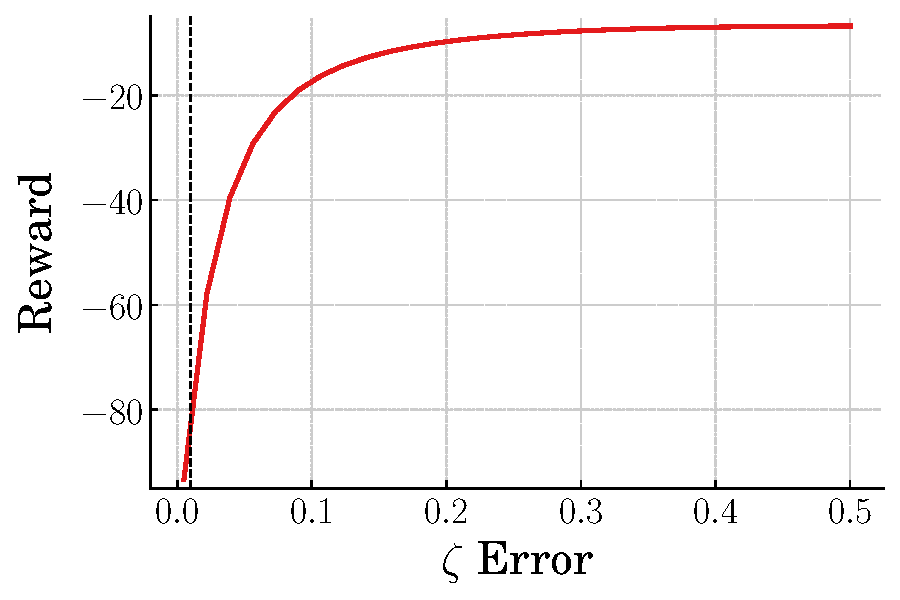
\includegraphics[width=\textwidth]{figures/figures_robustness/duffing_robustness/zeta_robustness_fixed_gain.pdf}
        \caption{$\zeta$}
        \label{subfig_chap4:duffing_zeta_robustness_fixed_gain}
    \end{subfigure}
       \caption{Robustness of model-based duffing oscillator controller}
       \label{fig_chap4:duffing_robustness_fixed_gain}
\end{figure}

\begin{figure}[t]
    \centering
    \begin{subfigure}[b]{0.49\textwidth}
        \centering
        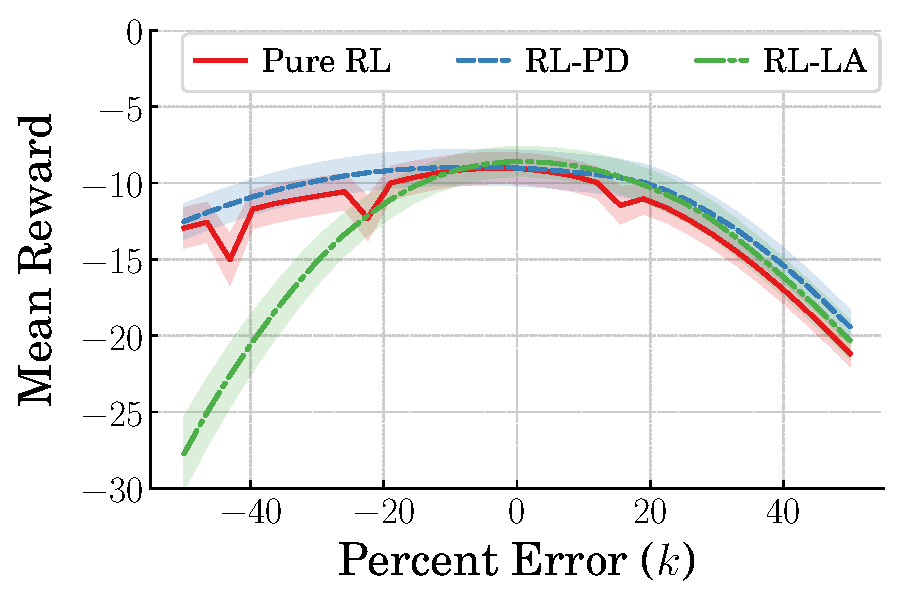
\includegraphics[width=\textwidth]{figures/figures_robustness/duffing_robustness/k_robustness.pdf}
        \caption{$k$}
        \label{subfig_chap4:duffing_k_robustness}
    \end{subfigure}\\
    \hfill
    \begin{subfigure}[b]{0.49\textwidth}
        \centering
        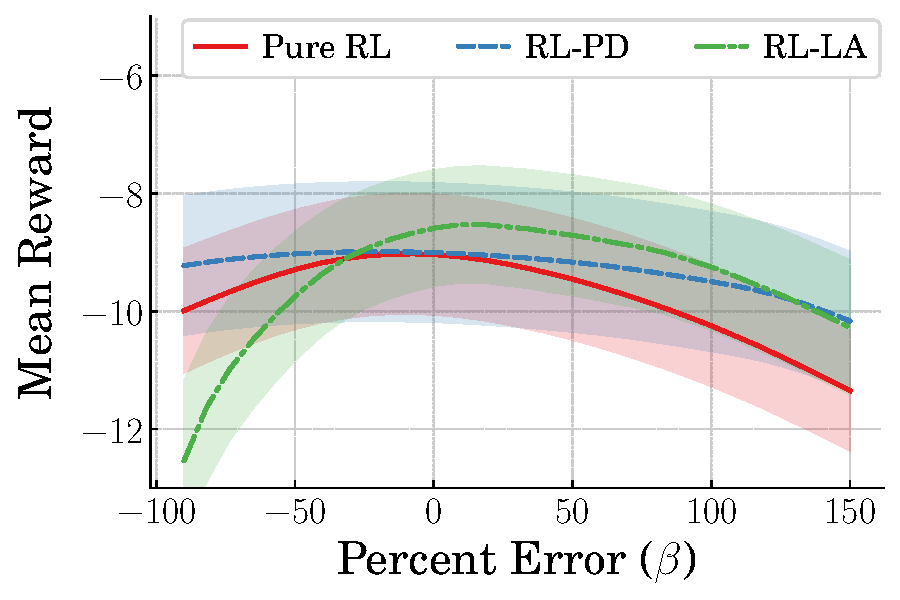
\includegraphics[width=\textwidth]{figures/figures_robustness/duffing_robustness/Beta_robustness.pdf}
        \caption{$\beta$}
        \label{subfig_chap4:duffing_Beta_robustness}
    \end{subfigure}
    \hfill
    \begin{subfigure}[b]{0.49\textwidth}
        \centering
        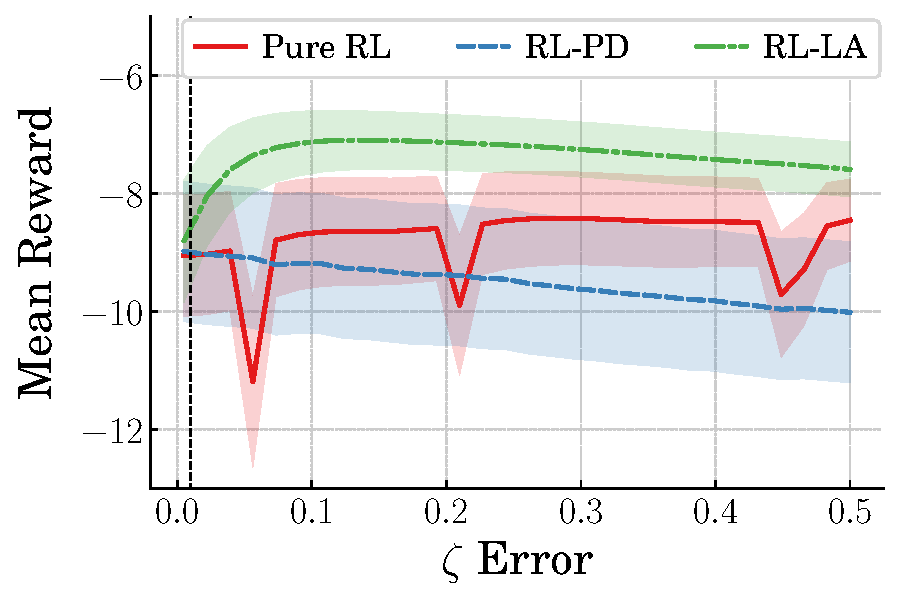
\includegraphics[width=\textwidth]{figures/figures_robustness/duffing_robustness/zeta_robustness.pdf}
        \caption{$\zeta$}
        \label{subfig_chap4:duffing_zeta_robustness}
    \end{subfigure}
       \caption{Robustness of RL and combined controllers to modeling error}
       \label{fig_chap4:duffing_robustness}
\end{figure}
%
\begin{figure}[tb]
    \centering
    \begin{subfigure}[b]{0.32\textwidth}
        \centering
        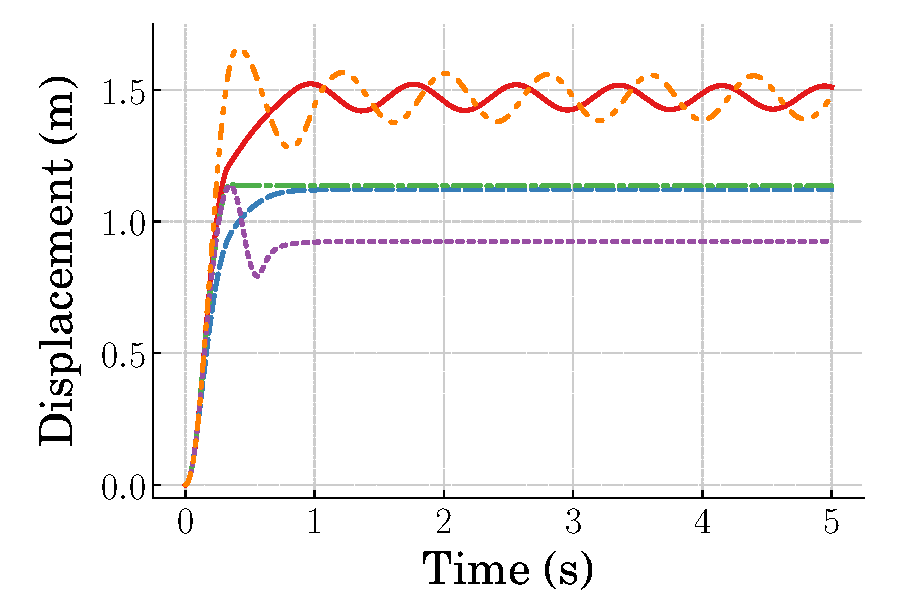
\includegraphics[width=\textwidth]{figures/figures_robustness/duffing_robustness/time_responses/0p5k_displacement.pdf}
        \caption{$-50\%$ error}
        \label{subfig_chap4:duffing_0p5k_displacement}
    \end{subfigure}
    \hfill
    \begin{subfigure}[b]{0.32\textwidth}
        \centering
        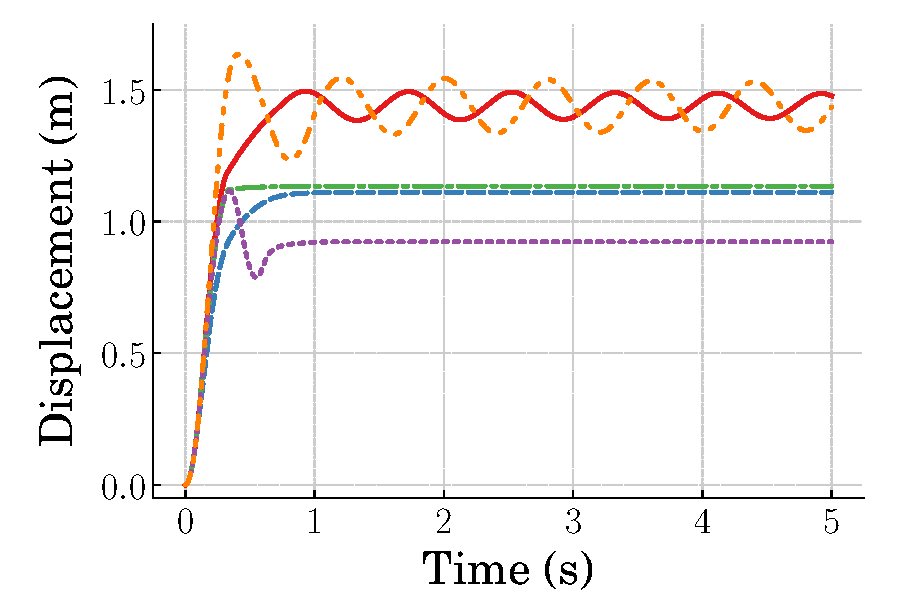
\includegraphics[width=\textwidth]{figures/figures_robustness/duffing_robustness/time_responses/1p0k_displacement.pdf}
        \caption{Nominal}
        \label{subfig_chap4:duffing_1p0k_displacement}
    \end{subfigure}
    \hfill
    \begin{subfigure}[b]{0.32\textwidth}
        \centering
        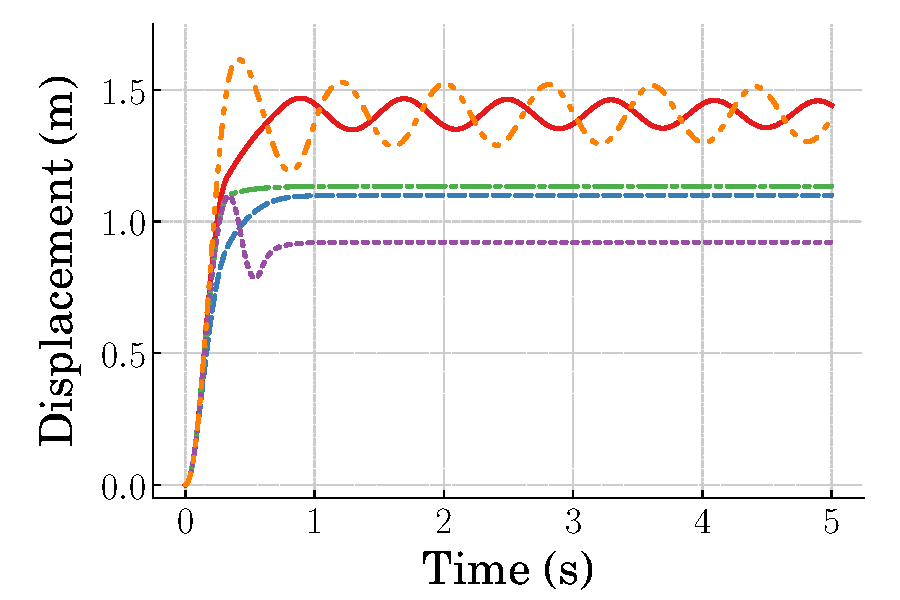
\includegraphics[width=\textwidth]{figures/figures_robustness/duffing_robustness/time_responses/1p5k_displacement.pdf}
        \caption{$+50\%$ error}
        \label{subfig_chap4:duffing_1p5k_displacement}
    \end{subfigure}
    \caption{RL-LA time responses for error in stiffness, $k$}
    \label{fig_chap4:duffing_k_error_responses}
  \end{figure}
  %
The plots in Figure~\ref{fig_chap4:duffing_robustness} show the sensitivity of the combined controllers to modeling error.
The mean reward was generated from the cumulative reward for the time response with each agent and controller type. The lines in each figure represent the mean reward and the shaded region is one standard deviation. 
%
Figure~\ref{subfig_chap4:duffing_k_robustness} shows the mean reward and standard deviation for linear stiffness modeling error, $k$. The mean reward decreases for all controllers as the modeling error increases. For modeling error less than the nominal stiffness, Pure RL and RL-PD have smaller rates of decrease in reward compared to RL-LA.
%
For stiffness modeling error greater than nominal stiffness, the different controllers have similar rates of decrease in mean reward. However, RL-PD tends to have the highest reward across most of the range of stiffness modeling error shown.
%
The rapid decrease in reward for RL-LA with lower than nominal stiffness is explained by Figure~\ref{fig_chap4:duffing_k_error_responses}, which shows time responses for $-50\%$, nominal, and $+50\%$ modeling error in stiffness. Two responses in Figure~\ref{subfig_chap4:duffing_0p5k_displacement} for $-50\%$ modeling error have higher steady-state error than the other cases.
%
For modeling error in $\beta$ in Figure~\ref{subfig_chap4:duffing_Beta_robustness}, the trends are similar to those shown for $k$ modeling error where RL-LA has the greatest sensitivity to $\beta$ that is lower than the nominal value. However, Pure RL has the highest sensitivity to $\beta$ greater than the nominal value.
%
Figure~\ref{subfig_chap4:duffing_zeta_robustness} shows the mean reward for a range of damping ratios. The controllers have less variation in mean reward from damping modeling error compared to modeling error in the stiffness parameters, $k$ and $\beta$. The reward with Pure RL tends to increase with increased damping ratio whereas the reward from RL-LA initially increases before gradually decreasing. The reward with RL-PD only decreases with increasing damping ratio due to the responses already being highly damped for the nominal damping ratio.


In general for the duffing oscillator controllers, the RL-PD controller had the greatest insensitivity to modeling error compared to Pure RL and RL-LA. RL-LA tended to be most sensitive to $k$ and $\beta$ values that were below the nominal values. However, the controllers still tend to perform well even for large modeling error.

\section{Double-Pendulum Crane Robustness}

\subsection{Modal Contributions}

The robustness of the double-pendulum crane controllers were evaluated for a range in hoist length, $l_1$, rigging length, $l_2$, and payload mass, $m_p$. The performance degradation from parameter variation can be the result of changes to the modes of oscillation and response amplitudes.
% For a system such as a crane, variation in the model may also be a result of intentional changes in configuration based on what is needed for its current application, such as changes in payload inertia or cable lengths.
% Additionally, for many systems, it may be necessary to intentionally change the configuration or physical parameters of the system to adapt to its current application.
% To investigate the sensitivity of the combined controllers to systems with various physical parameters, their performance was evaluated for simulated modeling error in hoist length, rigging length, and payload-to-hook-mass ratio.
%
The two modes of a linearized double-pendulum are~\cite{Blevins:1979a}:
%
\begin{equation}
\omega_{1,2}=\sqrt{\frac{g}{2}}\sqrt{(1+R)\left(\frac{1}{l_1}+\frac{1}{l_2}\right)\mp\beta}
\label{eq_chap4:modes}
\end{equation}
%
where $R$ is the payload-to-hook mass ratio and $\beta$ is:
%
\begin{equation}
\beta = \sqrt{(1+R)^2\left(\frac{1}{l_1}+\frac{1}{l_2}\right)^2-4\left( \frac{1+R}{l_1l_2}\right)}
\end{equation}
%
Assuming the amplitude of oscillation is low,
the total response amplitude from a unity magnitude impulse is the sum of the amplitude responses due to both angular displacements:
% the response of the endpoint from a unity magnitude impulse is:
%
\begin{equation}
A_{Total} = A_1 + A_2
\end{equation}
%
% where the response of the payload to a unity impulse is:
where
%
\begin{align}
A_1 = \frac{\omega_1l_1(1+{\omega_2}^2\alpha(l_1+l_2))}{k}\\
A_2 = \frac{\omega_2l_1(1+{\omega_1}^2\alpha(l_1+l_2))}{k}
\end{align}
\begin{align}
\alpha & = \frac{-g(1+R)}{{\omega_1}^2{\omega_2}^2l_1l_2}\\
k & = \beta l_1g
\end{align}


\begin{figure}[t]
     \centering
     \begin{subfigure}[b]{0.49\textwidth}
         \centering
         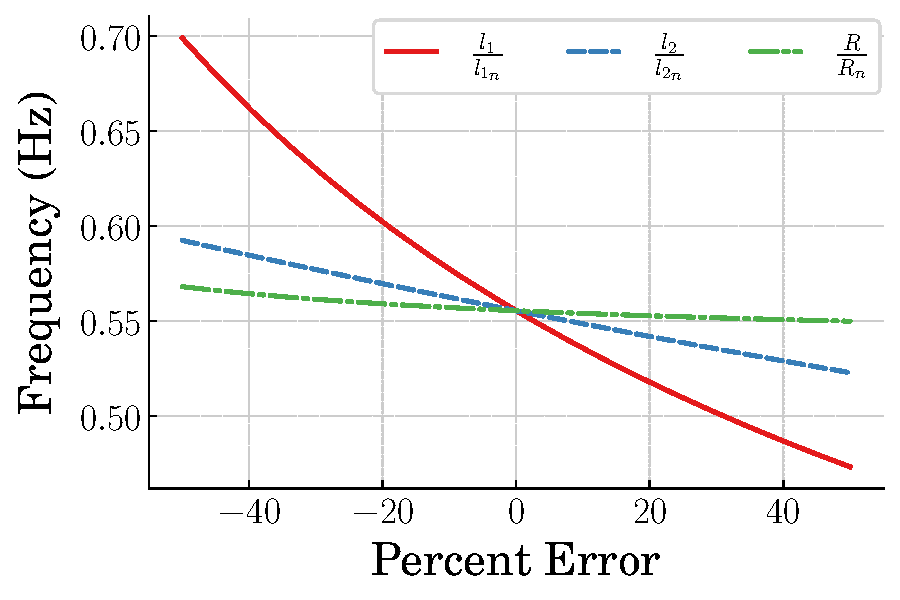
\includegraphics[width=\textwidth]{figures/figures_robustness/dpcrane_low_mode.pdf}
         \caption{Low mode}
         \label{subfig_chap4:dpcrane_low_mode}
     \end{subfigure}
     \hfill
     \begin{subfigure}[b]{0.49\textwidth}
         \centering
         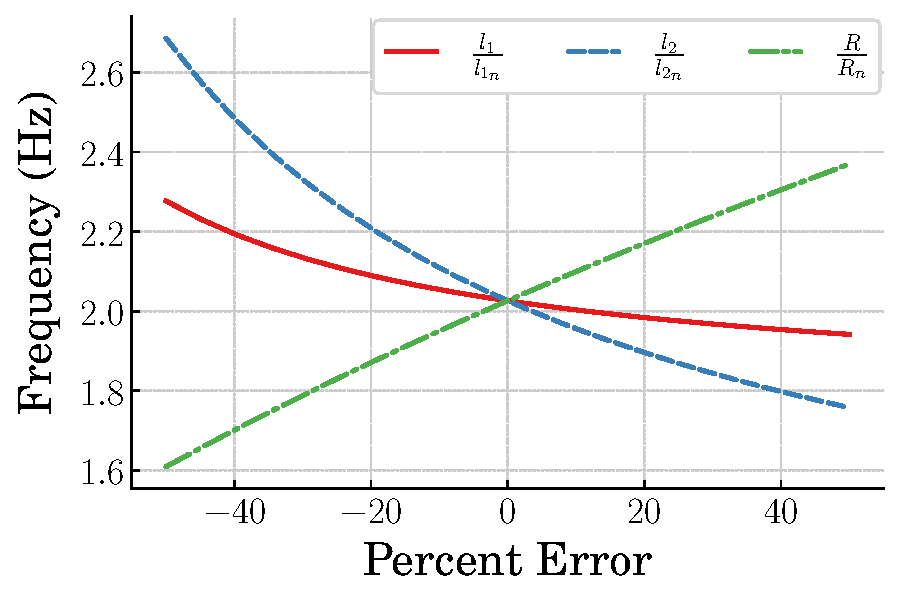
\includegraphics[width=\textwidth]{figures/figures_robustness/dpcrane_high_mode.pdf}
         \caption{High mode}
         \label{subfig_chap4:dpcrane_high_mode}
     \end{subfigure}
        \caption{Modes of crane vs. modeling error}
        \label{fig_chap4:dpcrane_modes}
\end{figure}

\begin{figure}[t]
     \centering
     \begin{subfigure}[b]{0.49\textwidth}
         \centering
         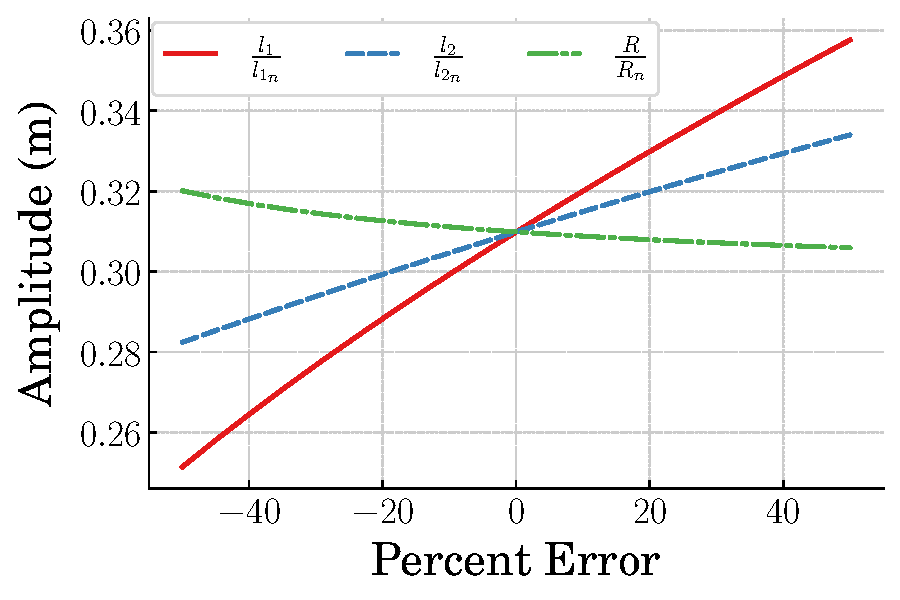
\includegraphics[width=\textwidth]{figures/figures_robustness/dpcrane_low_mode_amplitude.pdf}
         \caption{Low mode contribution amplitude}
         \label{subfig_chap4:dpcrane_low_mode_amplitude}
     \end{subfigure}
     \hfill
     \begin{subfigure}[b]{0.49\textwidth}
         \centering
         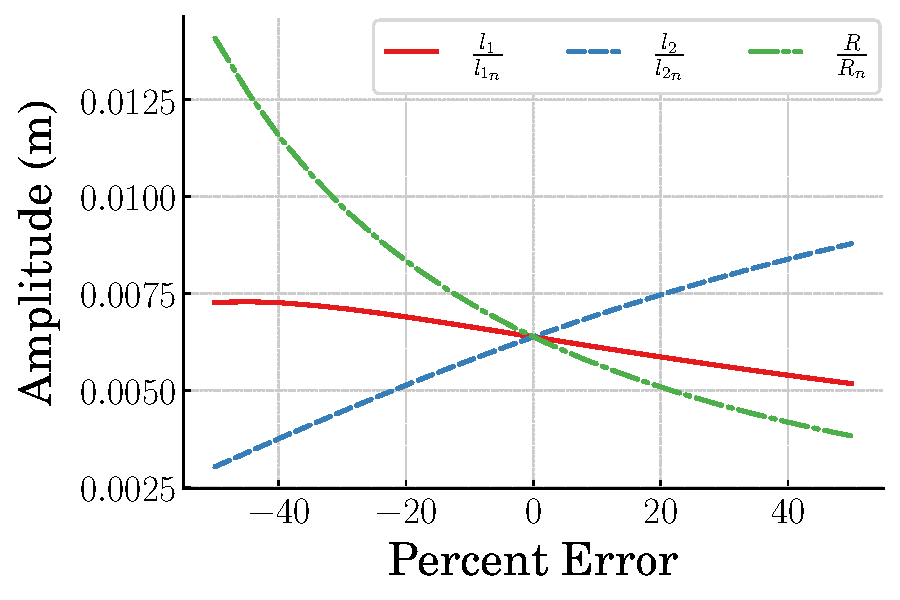
\includegraphics[width=\textwidth]{figures/figures_robustness/dpcrane_high_mode_amplitude.pdf}
         \caption{High mode contribution amplitude}
         \label{subfig_chap4:dpcrane_high_mode_amplitude}
     \end{subfigure}
        \caption{Amplitude contributions of crane modes}
        \label{fig_chap4:dpcrane_modes_amplitude}
\end{figure}

The change in the modes of the crane for modeling error is shown in Figure~\ref{fig_chap4:dpcrane_modes}. The variation in the low mode in Figure~\ref{subfig_chap4:dpcrane_low_mode} show that modeling error in hoist length, $l_1$ has the most significant effect on the low mode for the range of $\pm 50 \%$ modeling error. However, hoist length has the lowest effect on the high mode shown in Figure~\ref{subfig_chap4:dpcrane_high_mode}. Modeling error in rigging length, $l_2$, and payload-to-mass ratio, $R$, have the greatest effect on the high mode frequency.
%
The response amplitude from a unity magnitude impulse on a linearized double-pendulum is shown in Figure~\ref{fig_chap4:dpcrane_modes_amplitude}. The contribution from the low mode is most significantly affected by the hoist length, $l_1$, as shown in Figure~\ref{subfig_chap4:dpcrane_low_mode_amplitude}. This corresponds with the change in low-mode frequency. For the high-mode contribution in Figure~\ref{subfig_chap4:dpcrane_high_mode_amplitude}, payload-to-hook mass ratio, $R$, has the largest impact on the amplitude. Based on the changes in modal frequency and modal amplitude contributions, the most significant factors affecting performance degradation are modeling error in hoist length, $l_1$, and payload-to-hook mass ratio. The rest of this section discusses robustness of the double pendulum crane controllers to this modeling error.
%

% % This is the hammer
% \begin{table}[tb]
% \begin{center}
%   \setlength{\tabcolsep}{6pt}
%   \caption{Nominal Training Parameters}
%   \begin{tabular}{ c c c c }
%     \hline
%     $l_{1_n}$ & $l_{2_n}$ & $m_{p_n}$ & $m_{h_n}$\\ 
%    \hline
%     0.619125 & 0.247115 & 0.0949 & 0.0444\\
%   \label{table:baseline_experiments}
%   \end{tabular}
%   \end{center}
% \end{table}

\subsection{Crane Controller Robustness}

\begin{figure}[tb]
    \centering
    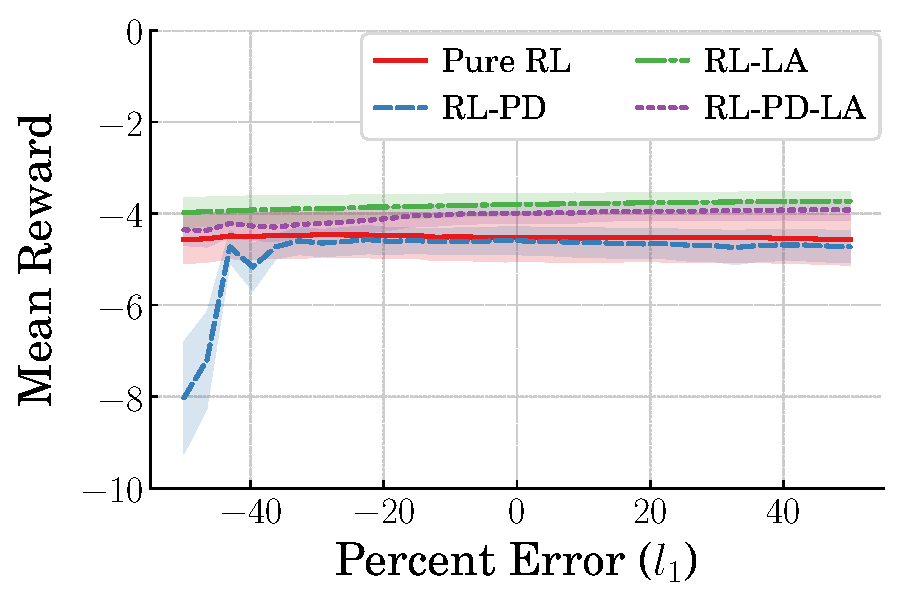
\includegraphics[width=0.65\columnwidth]{figures/figures_robustness/dpcrane_robustness/L1_robustness.pdf}
    \vspace{-2ex}
    \caption{Mean reward for a range of hoist lengths}
  % \vspace{-2ex}
    \label{fig:mean_reward_hoist_length}
\end{figure}
%
The agents discussed previously were trained with fixed parameters. The sensitivity of the controllers to modeling error was evaluated for the final weights during training at episode $3000$. The controllers were evaluated over a range of $\pm 50\%$ modeling error. Figure~\ref{fig:mean_reward_hoist_length} shows the mean and standard deviation of reward of the controllers for percent modeling error in hoist length, $l_1$.
% , where $l_{1_n}$ is the nominal hoist length used for training.
% Despite the changes in the low mode for modeling error in hoist length, the modeling error does not significantly affect the mean reward for the controllers.
The modeling error does not significantly affect the mean reward for most of the range shown. However, the mean reward from RL-PD is much lower for modeling error $40\%$ less than the nominal value.
%
\begin{figure}[tb]
    \centering
    \begin{subfigure}[b]{0.32\textwidth}
        \centering
        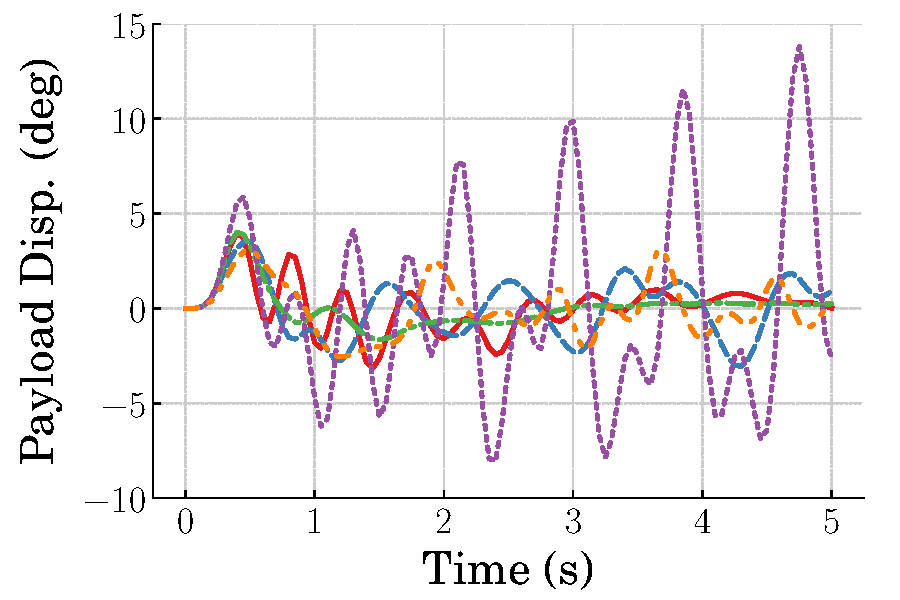
\includegraphics[width=\textwidth]{figures/figures_robustness/dpcrane_robustness/time_responses/0p5L1_payload.pdf}
        \caption{$-50\%$ error}
        \label{subfig_chap4:dpcrane_0p5L1_payload}
    \end{subfigure}
    \hfill
    \begin{subfigure}[b]{0.32\textwidth}
        \centering
        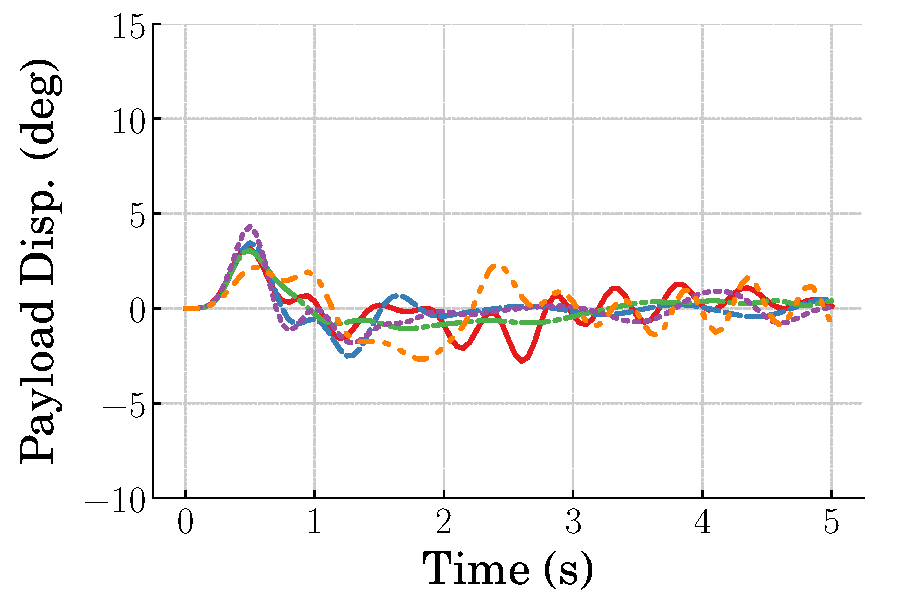
\includegraphics[width=\textwidth]{figures/figures_robustness/dpcrane_robustness/time_responses/1p0L1_payload.pdf}
        \caption{Nominal}
        \label{subfig_chap4:dpcrane_1p0L1_payload}
    \end{subfigure}
    \hfill
    \begin{subfigure}[b]{0.32\textwidth}
        \centering
        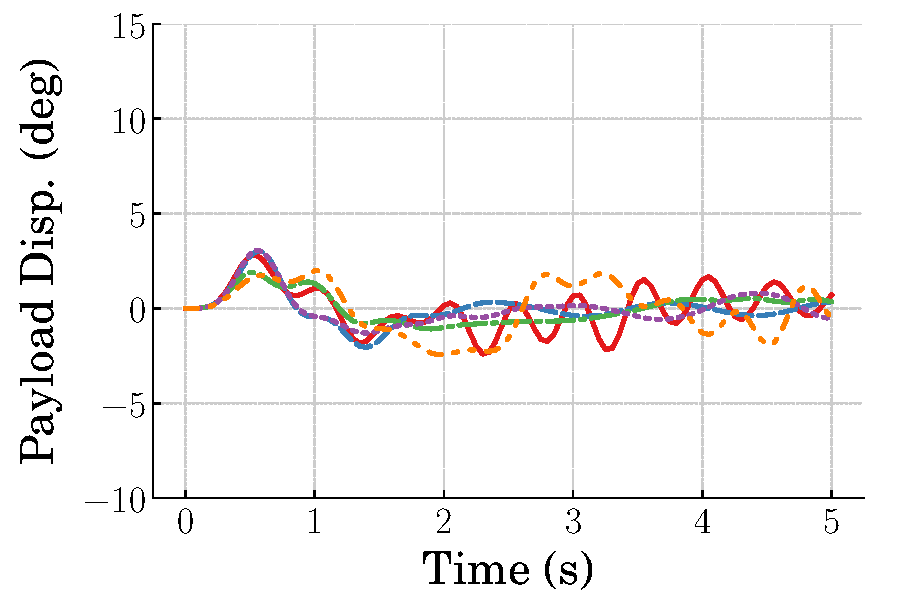
\includegraphics[width=\textwidth]{figures/figures_robustness/dpcrane_robustness/time_responses/1p5L1_payload.pdf}
        \caption{$+50\%$ error}
        \label{subfig_chap4:dpcrane_1p5L1_payload}
    \end{subfigure}
    \caption{RL-PD payload time responses for error in hoist length, $l_1$}
    \label{fig_chap4:dpcrane_hoist_error_responses}
  \end{figure}
  %
%
% \rnotes{Why? Possibly change in modal frequencies and RL-PD's tendency for residual oscillation?}
This decrease in reward is explained by the payload time responses with modeling error in hoist length shown in Figure~\ref{fig_chap4:dpcrane_hoist_error_responses}. The response amplitude for nominal hoist length in Figure~\ref{subfig_chap4:dpcrane_1p0L1_payload} is similar to the case with hoist length $50\%$ longer than nominal in Figure~\ref{subfig_chap4:dpcrane_1p5L1_payload}. The case with hoist length $50\%$ shorter than nominal has one response with growing amplitude that skews the mean of the reward.

\begin{figure}[tb]
    \centering
    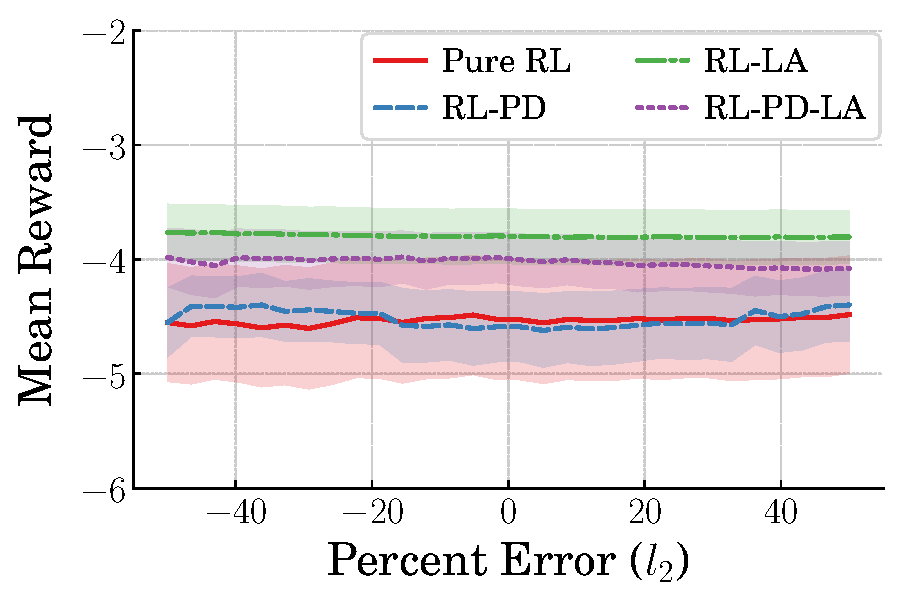
\includegraphics[width=0.65\columnwidth]{figures/figures_robustness/dpcrane_robustness/L2_robustness.pdf}
    \vspace{-2ex}
    \caption{Mean reward for a range of payload lengths}
  % \vspace{-2ex}
    \label{fig:mean_reward_payload_length}
\end{figure}
%
Although the controllers tend to have low sensitivity to hoist length modeling error, the reward from RL-LA and RL-PD-LA slightly increase with increasing hoist length whereas the reward from Pure RL and RL-PD slightly decrease.
% Although mean reward remains approximately the same, the standard deviation of the mean reward for the RL controller is higher than that of the two combined controllers.
%
Similarly, Figure~\ref{fig:mean_reward_payload_length} shows the change in reward for percent modeling error in rigging length, $l_2$.
% over the nominal length used in training, $l_{2_n}$.
All of the controllers show low sensitivity to rigging length. This was expected from the modal analysis, which showed that rigging length had less influence on modal contributions than other parameters.
%
\begin{figure}[tb]
    \centering
    % \includegraphics[width=\columnwidth]{figures/Mean_reward_v_hook_mass.pdf}
    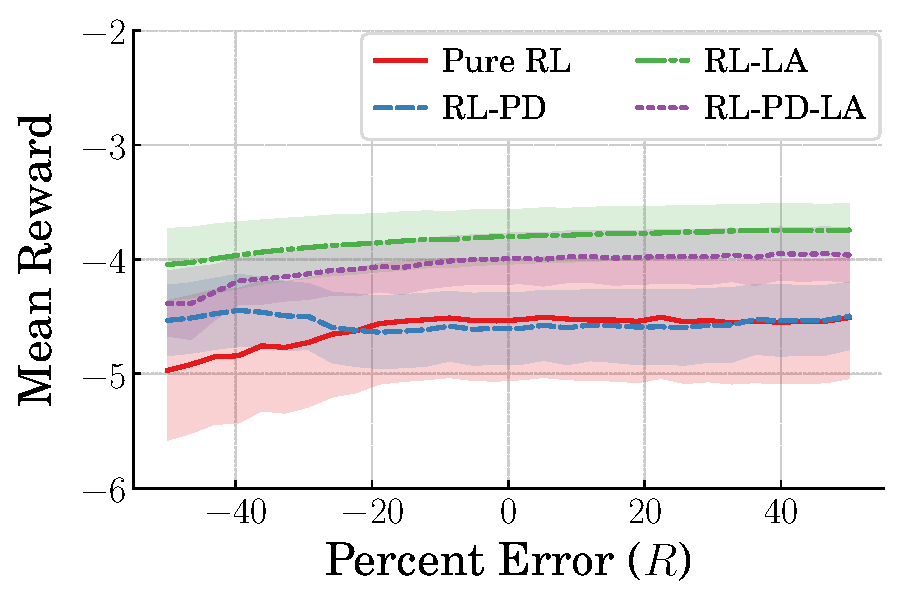
\includegraphics[width=0.65\columnwidth]{figures/figures_robustness/dpcrane_robustness/R_robustness.pdf}
    \vspace{-2ex}
    \caption{Mean reward for a range of mass ratios}
  % \vspace{-2ex}
    \label{fig:mean_reward_mass_ratio}
\end{figure}
The mean reward for payload mass modeling error, $R$, is shown in Figure~\ref{fig:mean_reward_mass_ratio}. The mean reward for most of the controllers tends to decrease as payload-to-hook mass decreases. However, the reward for RL-PD increased for payload-to-mass ratio less than the nominal value.
% \rnotes{Why?}
% Because the payload modeling error had little effect on the low mode of the system compared to changes in other parameters, the change in reward likely has other causes.
% \rph{such as changes in ratio of modal contribution?}
The standard deviation remains insensitive to modeling error for all parameters, with standard deviation from RL being higher than that of the combined controllers.

The hoist length, $l_1$, and payload-to-hook mass ratio, $R$, had the most significant impact on the mean reward from the controllers. However, despite the changing modal characteristics of the double-pendulum crane, the controllers tended to maintain low sensitivity to modeling error with RL-LA and RL-PD-LA having the lowest sensitivity.

\section{Inverted Pendulum Robustness}

This section presents a robustness analysis for the agents trained for the inverted pendulum. Since the previous sections have already presented robustness analysis for parametric modeling error, the robustness of inverted pendulum was evaluated for unmodeled dynamics.
Agents that were not able to cause the system to settle in the region of attraction in the ideal case were removed for the following robustness evaluation.

\subsection{Friction}

The agents were trained without friction in the ideal model. However, friction is a part of any physical system, and it is beneficial to determine the robustness of a controller to unmodeled friction. Since the input of the trolley was modeled as an acceleration input instead of a force, the friction was normalized by mass and modeled as an acceleration disturbance. The equation of motion of the inverted pendulum with coulomb friction is:
%
\begin{gather}
    \ddot{\theta} = (g\sin{\theta} + \cos{\theta} (\ddot{x}_d + f))/l\\
    f = \left\{
            \begin{array}{cl}
                - f_m \text{sgn}(\dot{x}) & \forall x \neq 0\\
                -\text{sat}^{f_m}_{-f_m}(\ddot{x}_d) & \dot{x} = 0
            \end{array}
    \right.
\end{gather}
%
where $f$ is the acceleration disturbance from normalized friction, and $f_m$ is the maximum disturbance magnitude. Stiction occurs when the velocity of the trolley is zero, $\dot{x}=0$, and friction is constant when the trolley is moving.
Figure~\ref{fig:friction_reward} shows the mean reward and standard deviation of the agents for a range of coulomb friction acting on the cart.
% Because the model uses an acceleration input, the friction is normalized by mass such that it can be modeled as a constant input disturbance.
%
For a range of normalized friction from $0$ to approximately $1.9\si[per-mode=symbol]{\newton\per\kilo\gram}$ the mean reward remains relatively unchanged as the agents are still capable of stabilizing the system. After this point, the mean reward begins decreasing more steeply for Pure RL and S-RL-LQR. At $2\si[per-mode=symbol]{\newton\per\kilo\gram}$, some of the S-RL-LQR agents begin to fail to stabilize the inverted pendulum, resulting in the decrease in mean reward. At $2.2\si[per-mode=symbol]{\newton\per\kilo\gram}$, some of the Pure RL agents begin failing to stabilize the system. After this, the mean reward for Pure RL is lower than that of the other controller types. However, all of the RL-LQR agents maintain the ability to stabilize the system for a larger range of normalized friction. The RL-LQR agents begin to fail to stabilize the system for normalized friction above $3.6\si[per-mode=symbol]{\newton\per\kilo\gram}$.


\begin{figure}[t]
    \centering
    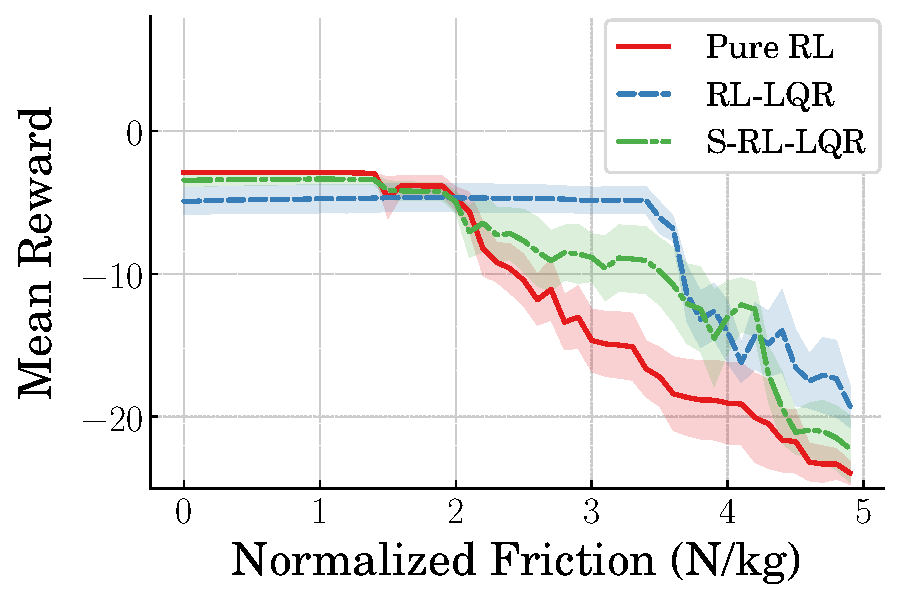
\includegraphics[scale=0.65]{figures/figures_robustness/invpend_robustness/friction_reward}
    \caption{Reward with normalized friction}
    \label{fig:friction_reward}
\end{figure}

\subsection{Feedback Noise}

Feedback noise is also a common occurrence when implementing sensors for feedback on a real system. Figure~\ref{fig:noise_reward} shows the mean reward from the agents when subjected to feedback noise. Noise was applied using a Gaussian distribution with a mean of $\mu=0$. Increasing the standard deviation of the distribution increases the severity of the added noise signal. Because the observation was normalized between $-1$ and $1$ during training, the noise signal was added to the normalized feedback signal.
%
The RL-LQR agents tend to have the lowest robustness to feedback noise compared to Pure RL and S-RL-LQR. The agents begin to fail to stabilize the system at noise standard deviation of $\sigma=0.025$. The Pure RL and S-RL-LQR agents begin to fail soon after this at $\sigma=0.03$, where two Pure RL agents and one S-RL-LQR agent fails during the simulation time. Between $\sigma=0.03$ and $\sigma=0.045$, only one of the S-RL-LQR agents have failed to achieve stability, whereas multiple of the Pure RL and RL-LQR agents have failed. Multiple S-RL-LQR agents begin to fail at $\sigma=0.045$, after which all agents fail to maintain stability for increasing noise severity.

% * 0.02 RL 0 fail, RL-LQR 0 fail, S-RL-LQR 0 fail
% * 0.025 RL 0 fail, RL-LQR 3 fail, S-RL-LQR 0 fail
% * 0.03 RL 2 fail, RL-LQR 3 fail, S-RL-LQR 1 fail
% * 0.035 RL 3 fail, RL-LQR 2 fail, S-RL-LQR 1 fail
% * 0.04 RL 4 fail, RL-LQR 4 fail, S-RL-LQR 1 fail
% * 0.045 RL 4 fail, RL-LQR 4 fail, S-RL-LQR 4 fail
% * 0.05 RL 4 fail, RL-LQR 4 fail, S-RL-LQR 5 fail

\begin{figure}[t]
    \centering
    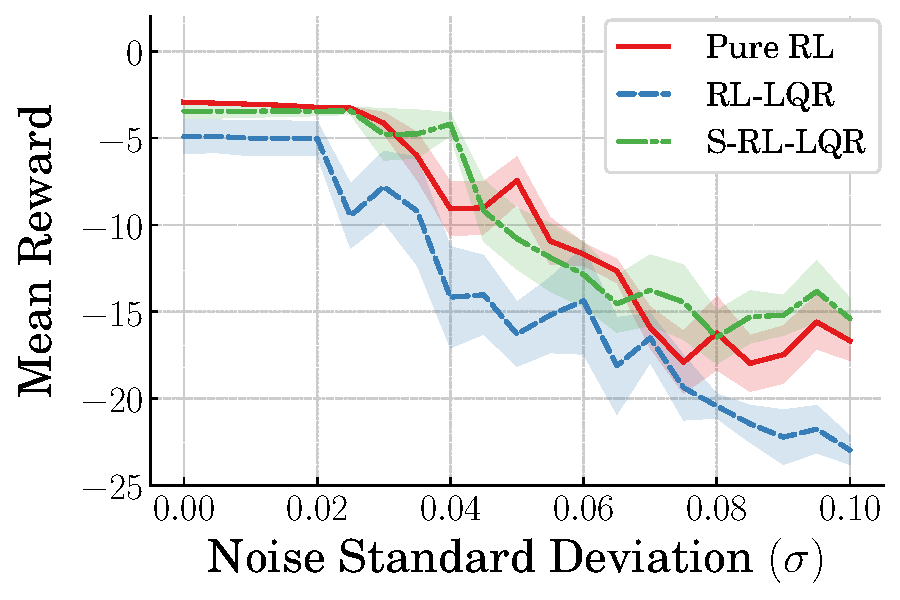
\includegraphics[scale=0.65]{figures/figures_robustness/invpend_robustness/noise_reward}
    \caption{Reward with observation noise}
    \label{fig:noise_reward}
\end{figure}

\subsection{Feedback Delay}

Delay is often introduced into a system as a result of required computation time for the controller.
Since the controllers in this work were trained and implemented with a fixed sampling rate, the simulated delay was modeled as multiples of the sampling time. Therefore, robustness was evaluated for multiple sampling rates.
%
Figure~\ref{fig_chap4:invpend_delay_reward} shows the mean reward and standard deviation for each controller type with delay.
%
% With a natural frequency of $1\si{\hertz}$ near the equilibriums, one delay step is $\frac{1}{20}$ of the system period.
%
The controllers with different sampling rates have similar trends in mean reward as delay increases. The controllers have low sensitivity to delays less than $0.05\si{\second}$, which was the sampling time used for training. The mean rewards begin to significantly decrease for delays greater than $0.05\si{\second}$. For longer delays, S-RL-LQR has the highest mean reward, whereas Pure RL has the lowest mean reward and highest standard deviation.
%
% Although mean reward from the various agents of each controller type are similar for no delay and a delay of one step, the mean reward decreases and the standard deviation increases at two delay steps, especially for the Pure RL controller. Both controllers combining RL and LQR were able to more easily maintain higher reward and lower standard deviation for the delay shown. 
% \rph{The high standard deviation is a result of some of the agents being unable to stabilize the system.}
%
\begin{figure}[tb]
  \centering
  \begin{subfigure}[b]{0.49\textwidth}
      \centering
      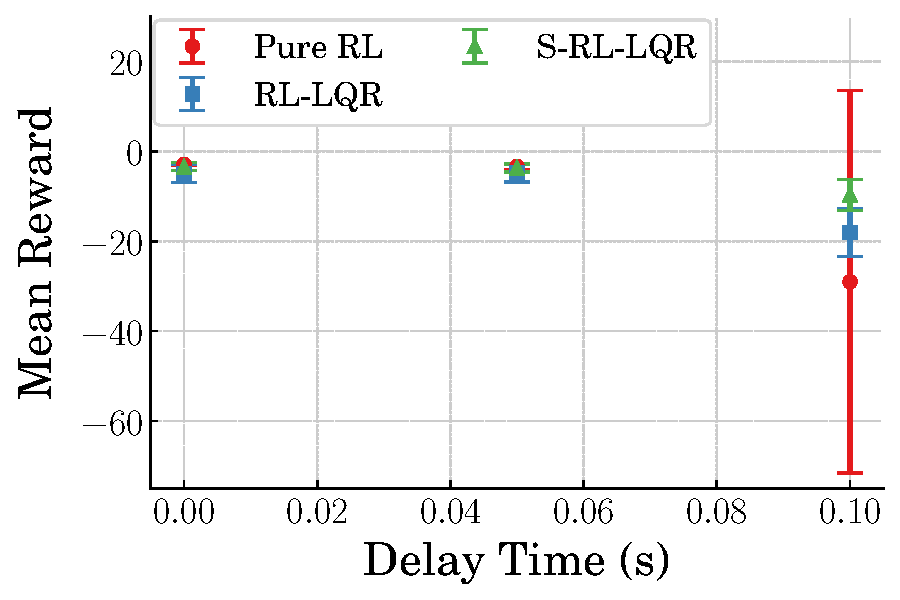
\includegraphics[width=\textwidth]{figures/figures_robustness/invpend_robustness/delay_reward_0.050_sampling.pdf}
      \caption{0.05\si{\second} sampling time}
      \label{subfig_chap4:invpend_reward_0.05}
  \end{subfigure}\\
  \hfill
  \begin{subfigure}[b]{0.49\textwidth}
      \centering
      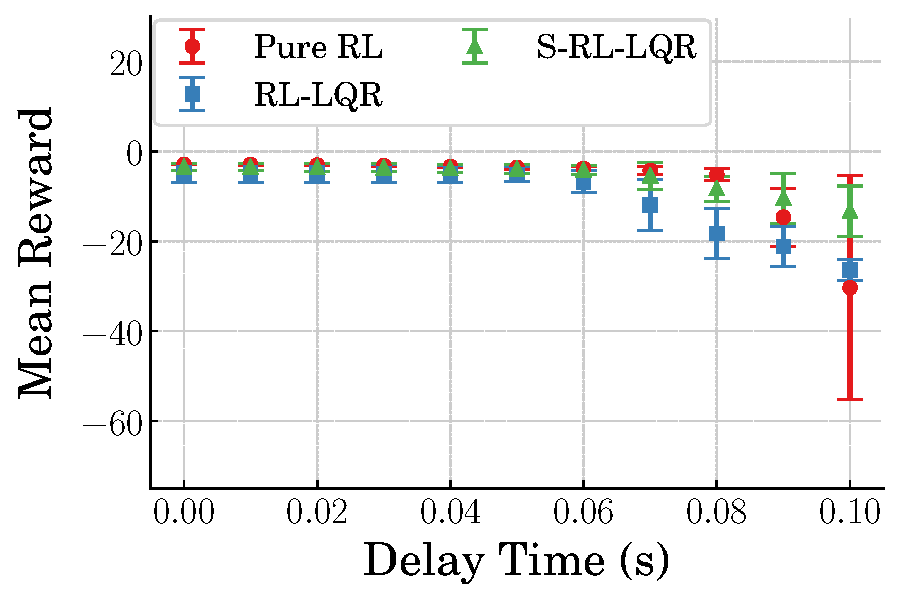
\includegraphics[width=\textwidth]{figures/figures_robustness/invpend_robustness/delay_reward_0.010_sampling.pdf}
      \caption{0.01\si{\second} sampling time}
      \label{subfig_chap4:invpend_delay_reward_0.01}
  \end{subfigure}
  \hfill
  \begin{subfigure}[b]{0.49\textwidth}
      \centering
      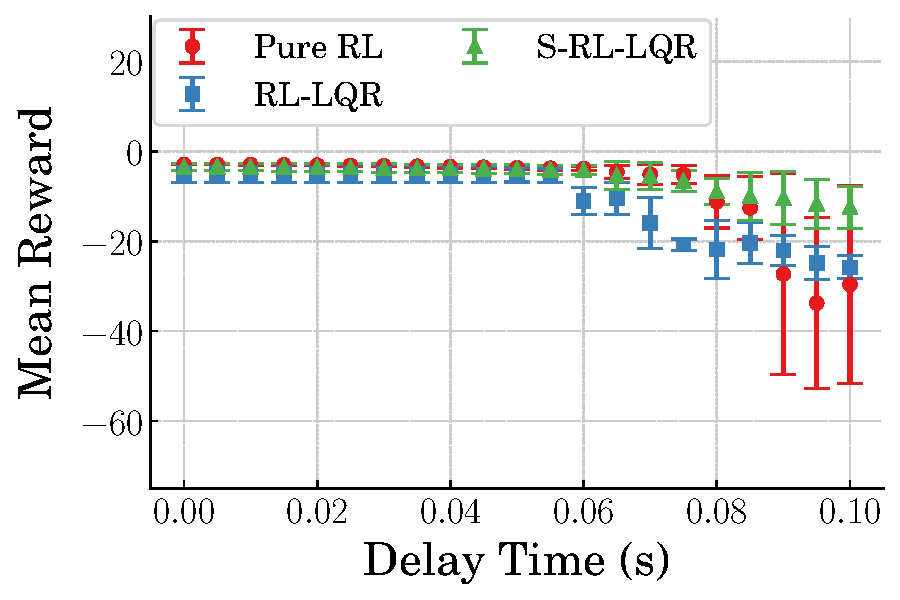
\includegraphics[width=\textwidth]{figures/figures_robustness/invpend_robustness/delay_reward_0.005_sampling.pdf}
      \caption{0.005\si{\second} sampling time}
      \label{subfig_chap4:invpend_delay_reward_0.005}
  \end{subfigure}
  \caption{Reward trends with time delays}
  \label{fig_chap4:invpend_delay_reward}
\end{figure}
%

%
\begin{figure}[tb]
    \centering
    \begin{subfigure}[b]{0.49\textwidth}
        \centering
        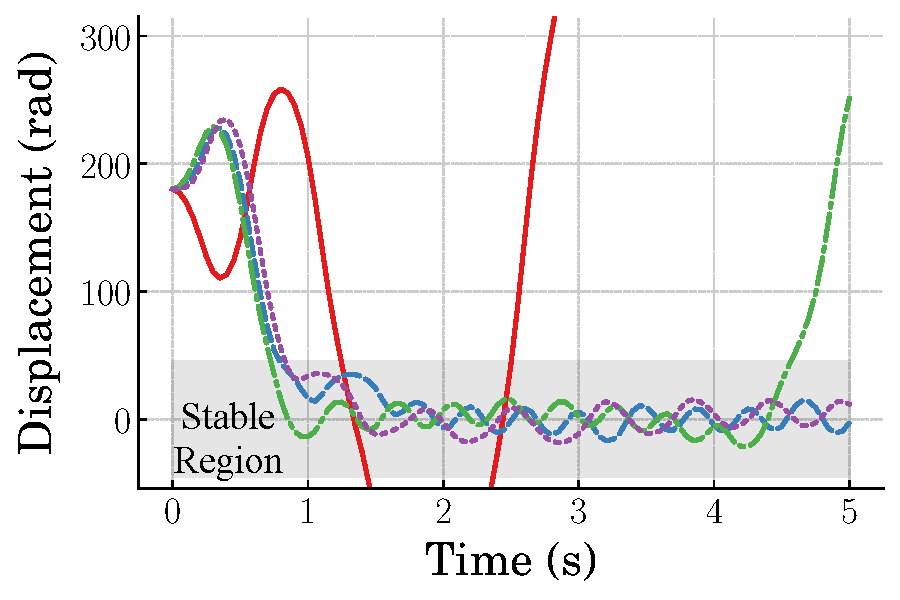
\includegraphics[width=\textwidth]{figures/figures_robustness/invpend_robustness/Angular_displacement_DELAY_2_pure_RL.pdf}
        \caption{Pure RL}
        \label{subfig_chap4:invpend_delay_pure_RL}
    \end{subfigure}\\
    \hfill
    \begin{subfigure}[b]{0.49\textwidth}
        \centering
        \includegraphics[width=\textwidth]{figures/figures_robustness/invpend_robustness/Angular_displacement_DELAY_2_lumped_LQR.pdf}
        \caption{RL-LQR}
        \label{subfig_chap4:invpend_delay_RL_LQR}
    \end{subfigure}
    \hfill
    \begin{subfigure}[b]{0.49\textwidth}
        \centering
        \includegraphics[width=\textwidth]{figures/figures_robustness/invpend_robustness/Angular_displacement_DELAY_2_switch_LQR.pdf}
        \caption{S-RL-LQR}
        \label{subfig_chap4:invpend_delay_S_RL_LQR}
    \end{subfigure}
    \caption{Angular displacement with $0.1\si{\second}$ delay}
    \label{fig_chap4:invpend_delay}
  \end{figure}
  %
Angular displacement time responses with a delay of $0.1\si{\second}$ and sampling time of $0.05\si{\second}$ are shown in Figure~\ref{fig_chap4:invpend_delay}.
The decrease in the mean reward and increase in standard deviation for the Pure RL controllers is a result of two of the agents diverging far from the equilibrium at $\theta=0$ as shown in Figure~\ref{subfig_chap4:invpend_delay_pure_RL}.
%
The remaining two agents successfully stabilize the inverted pendulum about the equilibrium.
% The agents that do not force the response to diverge to large values are successful at stabilizing the system about the desired displacement at $\theta=0$.
%
% \begin{figure}[t]
%     \centering
%     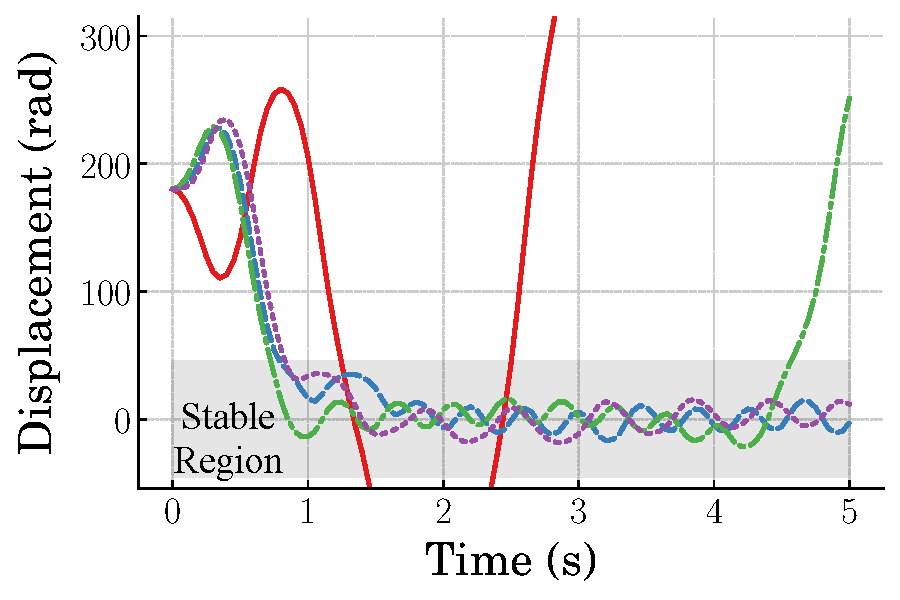
\includegraphics[scale=0.58]{figures/figures_robustness/invpend_robustness/Angular_displacement_DELAY_2_pure_RL}
%     \caption{Angular displacement using RL with delay of two time steps}
%     \label{fig:RL_disp_delay}
% \end{figure}
%
% Figure~\ref{subfig_chap4:invpend_delay_RL_LQR} shows the angular displacement response for the RL-LQR agents with a delay of two time steps.
Although the mean reward with RL-LQR was higher than that of Pure RL with the delay, fewer of the agents were able to stabilize the system as shown in Figure~\ref{subfig_chap4:invpend_delay_RL_LQR}. However, the responses that did not enter the stable region also did not diverge to displacements as large as those of Pure RL, resulting in the higher mean reward seen previously.
%
This is similar for the S-RL-LQR angular displacement responses for delay shown in Figure~\ref{subfig_chap4:invpend_delay_S_RL_LQR}. Only one of the agents was able to stabilize the system for the duration of the response. However, the unstable S-RL-LQR responses remained closer to the equilibrium than the unstable Pure RL responses.
% \rnotes{Figuring out how to summarize robustness of the inverted pendulum agents.}
%
% \begin{figure}[t]
%     \centering
%     \includegraphics[scale=0.58]{figures/figures_robustness/invpend_robustness/Angular_displacement_DELAY_2_lumped_LQR}
%     \caption{Angular displacement using RL-LQR with delay of two time steps}
%     \label{fig:RL_LQR_disp_delay}
% \end{figure}
% %
% \begin{figure}[t]
%     \centering
%     \includegraphics[scale=0.58]{figures/figures_robustness/invpend_robustness/Angular_displacement_DELAY_2_switch_LQR}
%     \caption{Angular displacement using S-RL-LQR with delay of two time steps}
%     \label{fig:S_RL_LQR_disp_delay}
% \end{figure}

In summary, the combined controllers for the inverted pendulum tended to have the least sensitivity to unmodeled friction compared to Pure RL. S-RL-LQR and Pure RL had the least sensitivity to high frequency noise compared to RL-LQR. For the cases with feedback delay, although more Pure RL responses tended to remain stable for a longer time period, the unstable responses from the combined controllers tended to remain closer to the equilibrium.

% \rnotes{Do I need this here.}
% \rph{Figure~\ref{fig_chap4:invpend_delay_init_180} shows the time responses with a delay of 0.1\si{\second} from an initial condition closer to the equilibrium, $\theta=20\si{\degree}$. This can help evaluate the robustness of the combined controllers within the region of attraction for LQR. The responses in Figure~\ref{subfig_chap4:invpend_delay_pure_RL_init_180} show that all but one of the Pure RL responses are stable with this feedback delay. The RL-LQR responses in Figure~\ref{subfig_chap4:invpend_delay_RL_LQR_init_180} have no responses that stay entirely in the stable region, although the response shown in red does return to the stable region. The S-RL-LQR responses in Figure~\ref{subfig_chap4:invpend_delay_S_RL_LQR_init_180} have only one stable response. Although the addition of a model-based controller with RL often provides improved performance, the addition of LQR for the inverted pendulum reduces the robustness of RL controllers to delay.}
% %
% \begin{figure}[tb]
%   \centering
%   \begin{subfigure}[b]{0.49\textwidth}
%       \centering
%       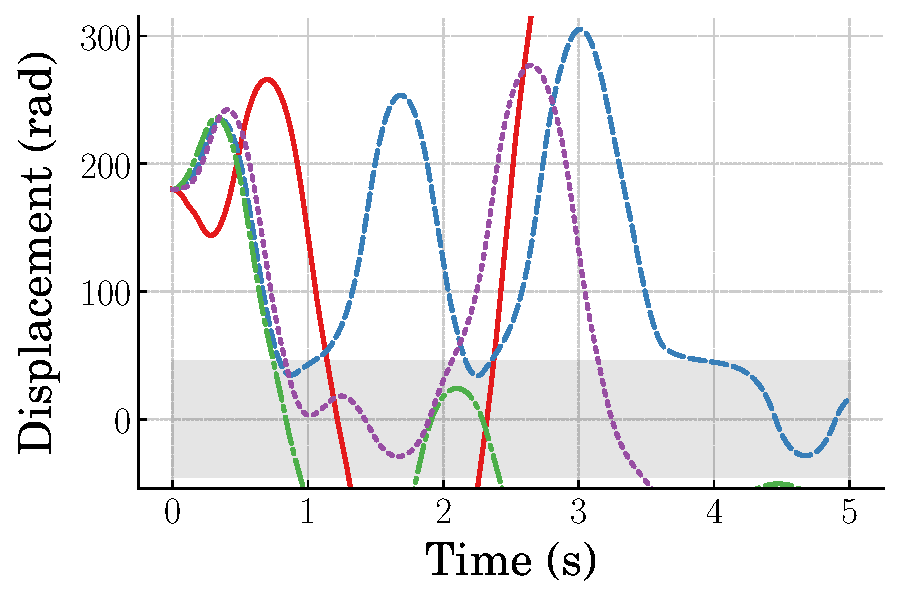
\includegraphics[width=\textwidth]{figures/figures_robustness/invpend_robustness/Angular_displacement_DELAY_20_pure_RL_init_180.pdf}
%       \caption{Pure RL}
%       \label{subfig_chap4:invpend_delay_pure_RL_init_180}
%   \end{subfigure}\\
%   \hfill
%   \begin{subfigure}[b]{0.49\textwidth}
%       \centering
%       \includegraphics[width=\textwidth]{figures/figures_robustness/invpend_robustness/Angular_displacement_DELAY_20_lumped_LQR_init_180.pdf}
%       \caption{RL-LQR}
%       \label{subfig_chap4:invpend_delay_RL_LQR_init_180}
%   \end{subfigure}
%   \hfill
%   \begin{subfigure}[b]{0.49\textwidth}
%       \centering
%       \includegraphics[width=\textwidth]{figures/figures_robustness/invpend_robustness/Angular_displacement_DELAY_20_switch_LQR_init_180.pdf}
%       \caption{S-RL-LQR}
%       \label{subfig_chap4:invpend_delay_S_RL_LQR_init_180}
%   \end{subfigure}
%   \caption{Angular displacement with delay of two time steps}
%   \label{fig_chap4:invpend_delay_init_180}
% \end{figure}
% %

\section{Conclusion}

Robustness of the combined controllers to modeling error was evaluated in this chapter. Each benchmark system had different places where modeling error could be introduced, and the modeling error was simulated for each system. The controllers for the duffing oscillator were evaluated with modeling error in stiffness and damping ratio. The Pure RL and combined controllers had high robustness to modeling error compared to the robustness of the fixed-gain controller alone, where Pure RL and RL-PD were the least sensitive to modeling error. For the double-pendulum crane, modeling error in hoist length, rigging length, and payload-to-hook mass ratio were introduced. The controllers for the crane tended to have low sensitivity to modeling error in all parameters except for the sensitivity of RL-PD to short rigging lengths. For the inverted pendulum, friction, feedback noise, and feedback delay were introduced to the system. Both combined controllers had more robustness to friction than Pure RL, with RL-LQR being the most robust. S-RL-LQR had the highest robustness to feedback noise. Although the combined controllers tended to have less sensitivity to friction and feedback noise, Pure RL tended to have the most robustness to feedback delay.

% \begin{itemize}
%     \item Duffing
%     \begin{itemize}
%         \item Agents had good robustness compared to robustness with only model-based control component
%         \item Pure RL and RL-PD were most insensitive to modeling error
%     \end{itemize}
%     \item Crane
%     \begin{itemize}
%         \item Generally high insensitivity for all modeling error
%         \item Only RL-PD was sensitive to low hoist length $l_1$
%     \end{itemize}
%     \item Inverted Pendulum
%     \begin{itemize}
%         \item Combined controllers were more robust to friction than RL-alone, with RL-LQR being the most robust
%         \item S-RL-LQR most robust to noise
%         \item Pure RL had better robustness to delay (sometimes)
%     \end{itemize}
% \end{itemize}

% \rph{In most cases, the combined controllers had comparable robustness to the Pure RL controllers.}